\pdfoutput=1
\documentclass[a4paper,pdftex]{article}
% \usepackage[whole]{bxcjkjatype}
\usepackage[T1]{fontenc}
\usepackage{tgtermes}

% ---Display \subsubsection at the Index
\setcounter{tocdepth}{3}

% ---Setting about the geometry of the document----
\usepackage{a4wide}
% \pagestyle{empty}

% ---Physics and Math Packages---
\usepackage{amssymb, amsfonts, amsthm, mathtools}
\usepackage{physics, braket, bm}
\usepackage{slashed}

% ---underline---
\usepackage{ulem}

% ---cancel---
\usepackage{cancel}

% --- surround the texts or equations
% \usepackage{fancybox,ascmac}

% ---settings of theorem environment---
% \theoremstyle{definition}
% \newtheorem{dfn}{Definition}
% \newtheorem{prop}{Proposition}
% \newtheorem{thm}{Theorem}

% ---settings of proof environment---
% \renewcommand{\proofname}{\textbf{Proof}}
% \renewcommand{\qedsymbol}{$\blacksquare$}

% ---Ignore the Warnings---
\usepackage{silence}
\WarningFilter{latexfont}{Some font shapes,Font shape}
\ExplSyntaxOn
\msg_redirect_name:nnn{hooks}{generic-deprecated}{none}
\ExplSyntaxOff

% ---Insert the figure (If insert the `draft' at the option, the process becomes faster.)---
% \usepackage{graphicx}
% \usepackage{subcaption}

% ----Add a link to a text---
\usepackage{url,hyperref}
\usepackage[dvipsnames,svgnames]{xcolor}
\hypersetup{colorlinks=true,citecolor=FireBrick,linkcolor=Navy,urlcolor=purple}
% \usepackage[whole,autotilde]{bxcjkjatype}

% ---Tikz---
\usepackage{tikz,pgf,pgfplots,circuitikz}
\pgfplotsset{compat=1.15}
\usetikzlibrary{intersections, arrows.meta, angles, calc, 3d, decorations.pathmorphing}
\usepackage[compat=1.1.0]{tikz-feynhand}

% ---Add the section number to the equation, figure, and table number---
\makeatletter
   \renewcommand{\theequation}{\thesection.\arabic{equation}}
   \@addtoreset{equation}{section}
   
   \renewcommand{\thefigure}{\thesection.\arabic{figure}}
   \@addtoreset{figure}{section}
   
   \renewcommand{\thetable}{\thesection.\arabic{table}}
   \@addtoreset{table}{section}
\makeatother

% ---enumerate---
% \renewcommand{\labelenumi}{$\arabic{enumi}.$}
% \renewcommand{\labelenumii}{$(\arabic{enumii})$}

% ---Index---
% \usepackage{makeidx}
% \makeindex 

% ---Fonts---
% \renewcommand{\familydefault}{\sfdefault}

% ---Title---
\title{My Study Notes 2024 / QFT ver.}
\author{Miyane}
\date{Last modified:\ \today}

\begin{document}

\maketitle

\tableofcontents

\clearpage

\section{Einstein–Cartan spacetime}

When we consider the effect of gravity, we have to introduce the notion of curved space. In this section, I would like to note mathematical tools for the theory of general relativity.

\subsection{Connection and  Torsion}

Covariant derivative:
\begin{align}
  \nabla_{\nu}A_{\mu}(x)
  &\equiv
  \partial_{\nu}A_{\mu}(x)
  -
  \Gamma^{\lambda}_{\ \mu\nu}(x)A_{\lambda}(x)
  \ ,\ 
  \\
  \nabla_{\nu}A^{\mu}(x)
  &\equiv
  \partial_{\nu}A^{\mu}(x)
  +
  \Gamma^{\mu}_{\ \lambda\nu}(x)A^{\lambda}(x)
\end{align}
where $\Gamma^{\lambda}_{\ \mu\nu}$ are \textit{Affine connections} which define the parallel transport of covariant vector fields as
\begin{equation}
  A_{\mu}(x+\dd x \parallel x)
  \equiv
  A_{\mu}(x)
  +
  \Gamma^{\lambda}_{\ \mu\nu}A_{\lambda}(x)\dd x^{\nu}
  .
\end{equation}

A metric $g_{\mu\nu}(x)$ satisfies the \textit{metric condition}
\begin{equation}
  \nabla_{\lambda}g_{\mu\nu}
  =
  0
  \ .
\end{equation}
















\clearpage

\section{Supersymmetry and Supergravity}






















\clearpage
\section{Renormalization and Effective Field Theory}






\clearpage
\section{Quantization of the gauge theory}

Reference: Chapter 9 and 16 of Peskin's textbook\cite{Peskin_IntroductionQuantum_1995}.

\subsection{Quantization of the Electromagnetic Field}

We will review the quantization of the Electromagnetic Field by the path integral method. We can write the action of the kinetic term as 
\begin{equation}
  S
  =
  \int\dd^4x \left[ -\frac{1}{4}F^{\mu\nu}F_{\mu\nu} \right]
\end{equation}
where $F_{\mu\nu}=\partial_{\mu}A_{\nu}-\partial_{\nu}A_{\mu}$. We will rewrite this Lagrangian as 
\begin{align}
  \int\dd^4x \left[ -\frac{1}{4}F^{\mu\nu}F_{\mu\nu} \right]
  &=
  -\frac{1}{2}
  \int\dd^4x
  (\partial_{\mu}A_{\nu}\partial^{\mu}A^{\nu}-\partial_{\nu}A_{\mu}\partial^{\mu}A^{\nu})
  \nonumber
  \\
  &=
  \frac{1}{2}
  \int\dd^4x\ 
  A_{\mu}(x)
  (\partial^2g^{\mu\nu}A_{\nu}(x)-\partial^{\mu}\partial^{\nu}A_{\nu}(x))
  \nonumber
  \\
  &=
  \frac{1}{2}\int\dd^4 x\int\frac{\dd^4 k'}{(2\pi)^4}\int\frac{\dd^4 k}{(2\pi)^4}e^{-i(k+k')\cdot x}
  \tilde{A}_{\mu}(k')
  (k^{\mu}k^{\nu}-g^{\mu\nu}k^2)
  \tilde{A}_{\nu}(k)
  \nonumber
  \\
  &=
  \frac{1}{2}
  \int\frac{\dd^4 k}{(2\pi)^4}
  \tilde{A}_{\mu}(-k)
  (k^{\mu}k^{\nu}-g^{\mu\nu}k^2)
  \tilde{A}_{\nu}(k)
  \ .
\end{align}
Note that we integrated by parts at the second equality and did a Fourier transformation of the field as
\begin{equation}
  A_{\mu}
  =
  \int\frac{\dd^4 k}{(2\pi)^4}
  \tilde{A}_{\mu}(k)e^{-ik\cdot x}
\end{equation}
at the third equality.

The functional integral
\begin{equation}
  Z
  \overset{?}{=}
  \int\mathcal{D}A\ 
  e^{iS[A]}
  \nonumber
\end{equation}
will diverge if we choose the gauge $\tilde{A}_{\mu}=k_{\mu}\alpha(x)$ where $\alpha(x)$ is a arbitrarily scalar function. Such a difficulty comes from the gauge invariance\footnote{
  Equivalently, the equation
  $$
    (-k^2g_{\mu\nu}+k_{\mu}k_{\nu})\tilde{D}_{F}^{\nu\rho}(k)
    =
    i\delta_{\mu}^{\rho}
  $$
  which define the Feynman propagator$\tilde{D}_{F}^{\mu\nu}(k)$ has no solution. This also caused such difficulty.
}. 

We can avoid this difficulty using a trick due to Faddeev and Popov. Let $G(A)$ be some function of $A^{\mu}$ and we wish to set it equal to zero as a gauge fixing condition; e.g. $G(A)=\partial_{\mu}A^{\mu}$ corresponds to Lorenz gauge. 

For any discontinuous filed $\bm{g}=(g_{1},\cdots,g_{n})$, the identity
\begin{equation}
  1
  =
  \int \prod_{i}\dd g_{i}
  \delta(\bm{g})
\end{equation} 
holds. If we transform fields $\bm{g}$ to fields $\bm{a}=(a_{1},\cdots,a_{n})$, we get the equality
\begin{equation}
  1
  =
  \int\left( \prod_{i}\dd a_{i} \right)
  \delta(\bm{g}(\bm{a}))\det\left( \pdv{\bm{g}}{\bm{a}} \right)
  .
\end{equation}

Generalizing discontinuous cases to the continuous cases, we find the identity in the following form:
\begin{equation}
  1
  =
  \int\mathcal{D}\alpha(x)\ 
  \delta(G(A^{\alpha}))
  \det\left( \frac{\delta G(A^{\alpha})}{\delta\alpha} \right)
  \ ,
\end{equation}
where $A^{\alpha}$ denotes the gauge-transformed field
\begin{equation}
  A_{\mu}^{\alpha}(x)
  =
  A_{\mu}
  +
  \frac{1}{e}\partial_{\mu}\alpha(x)
\end{equation}
and we regard $A^{\alpha}_{\mu}$ as the different field than $A_{\mu}$.

We insert 1 into the functional integral
\begin{align}
  \int\mathcal{D}A\ e^{iS[A]}
  &=
  \int\mathcal{D}A\int\mathcal{D}\alpha\ 
  \delta(G(A^{\alpha}))
  \underbrace{\det\left( \frac{\delta G(A^{\alpha})}{\delta \alpha} \right)}_{\text{no}\ \alpha\ \text{and}\ A}e^{iS[A]}
  \nonumber
  \\
  &=
  \det\left( \frac{\delta G(A^{\alpha})}{\delta \alpha} \right)
  \int\mathcal{D}A\int\mathcal{D}\alpha\ 
  \delta(G(A))e^{iS[A]}
  \ .
\end{align}
The functional determinant is evaluated as
\begin{equation}
  \det\left( \frac{\delta G(A^{\alpha})}{\delta \alpha} \right)
  =
  \det\left( \frac{1}{e}\partial^2 \right)
\end{equation}
since $G(A^{\alpha})=\partial^{\mu}A_{\mu}+\partial^2\alpha/e$. 

If we choose gauge fixing function $G(A$) as the general class functions
\begin{equation}
  G(A)
  =
  \partial_{\mu}A^{\mu}(x)-\omega(x)
\end{equation}
where $\omega(x)$ can be any scalar function, we obtain
\begin{equation}
  \int\mathcal{D}A\ e^{iS[A]}
  =
  \det\left( \frac{1}{e}\partial^2 \right)
  \int\mathcal{D}\alpha
  \int\mathcal{D}A\ 
  e^{iS[A]}\delta(\partial^{\mu}A_{\mu}(x)-\omega(x))
  .
\end{equation}
This relation holds for any $\omega(x)$. Thus we will integrate for all $\omega(x)$ to remove it and we insert the identity
\begin{equation}
  1
  =
  N(\xi)
  \int\mathcal{D}\omega(x)\ 
  \exp\left[ -i\int\dd^4 x\ \frac{\omega^2}{2\xi} \right]
\end{equation}
where $N(\xi)$ is an unimportant normalization constant depending on the parameter $\xi$. Finally, we obtain
\begin{equation}  
  \int\mathcal{D}A\ e^{iS[A]}
  =
  N(\xi)
  \det\left( \frac{1}{e}\partial^2 \right)
  \int\mathcal{D}\alpha
  \int\mathcal{D}A\ 
  e^{iS[A]}
  \exp\left[  
    -i\int\dd^4 x\ \frac{1}{2\xi}(\partial_{\mu}A^{\mu}(x))^2
  \right]
\end{equation}
by inserting the 1. 

We put this form into the generating function. It becomes
\begin{equation}
  Z[J^{\mu}]
  =
  \int\mathcal{D}A\ 
  \exp\left[  
    i\int\dd^4x\ 
    \left(  
      \frac{1}{2}A_{\mu}\left\{ g^{\mu\nu}\partial^2-\left( 1-\frac{1}{\xi} \right)\partial^{\mu}\partial^{\nu}\right\}A_{\nu} 
      +
      J^{\mu}A_{\mu}
    \right)
  \right]
  \ .
\end{equation}
Following the set stones, we shift the configuration as
\begin{equation}
  A_{\mu}
  \rightarrow
  A_{\mu}
  -
  \left\{ g_{\mu\nu}\partial^2-\left( 1-\frac{1}{\xi} \right)\partial_{\mu}\partial_{\nu}\right\}^{-1}J^{\nu}
\end{equation}
and we assume this shift does not change the measure $\mathcal{D}A$. Then we find
\begin{align}
  Z[J]
  &=
  \int\mathcal{D}A\ \exp\left[  
    i\int\dd^4x\ 
    \left\{  
      \frac{1}{2}(A_{\mu}-\{\cdots_{\mu}^{\ \rho}\}^{-1}J_{\rho} )(\cdots^{\mu\nu})(A_{\nu}-\{\cdots_{\nu}^{\ \sigma}\}^{-1}J_{\sigma} )
    \right.
  \right.
  \nonumber
  \\
  &\hspace*{3cm}
  \left.
    \left.
      +
      J^{\mu}
      (A_{\mu}-\{\cdots_{\mu}^{\ \rho}\}^{-1}J_{\rho} )
    \right\}
  \right]
  \nonumber
  \\
  &\equiv
  Z[J=0]
  \exp\left[  
    -\frac{i}{2}\int\dd^4x\int\dd^4 y\ 
    J_{\mu}(x)[-iD_{F}^{\mu\nu}(x-y)]J_{\nu}(y)
  \right]
\end{align}
where we put Feynman propagator
\begin{equation}
  -i\int\dd^4y\ D_{F}^{\mu\nu}(x-y)J_{\nu}(y)
  \equiv  
  \left\{ g^{\mu\nu}\partial^2-\left( 1-\frac{1}{\xi} \right)\partial^{\mu}\partial^{\nu}\right\}^{-1}J_{\nu}(x)
  \label{def_photon-propagator}
\end{equation}
since the functional derivative
\begin{equation}
  D_{F}^{\mu\nu}(x-y)
  =
  \frac{1}{Z_{0}}
  \left( -i\frac{\delta}{\delta J_{\mu}(x)} \right)
  \left( -i\frac{\delta}{\delta J_{\nu}(y)} \right)
  Z[J]
  \left.\vphantom{\frac{1}{2}}\right|_{J=0}
\end{equation}
guarantees \eqref{def_photon-propagator}. Thus we find the propagator for the momentum space
\begin{equation}
  \left(  
    -k^2 g_{\mu\nu}
    +
    \left( 1-\frac{1}{\xi} \right)k_{\mu}k_{\nu}
  \right)
  \tilde{D}_{F}^{\nu\rho}
  =
  i\delta_{\mu}^{\rho}
\end{equation}
and it is solved as
\begin{equation}
  \tilde{D}_{F}^{\mu\nu}
  =
  \frac{-i}{k^2+i\varepsilon}
  \left(  
    g^{\mu\nu}
    -
    (1-\xi)\frac{k^{\mu}k^{\nu}}{k^2}
  \right)
  \ .
\end{equation}

\subsubsection*{Summary}

\begin{itemize}
  \item 
  When quantizing the gauge theory, we should be careful of the gauge invariance. 
  \item 
  Due to such a property, the ill-defined divergence occurs in path integration, then we added the Faddeev-Popov term, parametrized by $\xi$, to converge the integral.
  \item 
  The $S$-matrix does not depend on the additional parameter $\xi$, thus it is unphysical. 
\end{itemize}

\subsection{Interactions of Non-Abelian Gauge Bosons}

We will check the following contents:
\begin{itemize}
  \item 
  guess Feynman rules.
  \item 
  check the Ward identities
  \item
  cancellation of the Amplitude to produce other photon polarization mode
\end{itemize}

\subsubsection*{Feynman rules}

The Yang-Mills Lagrangian is 
\begin{equation}
  \mathcal{L}
  =
  -
  \frac{1}{4}(F^{a}_{\mu\nu})^2
  +
  \bar{\psi}(i\slashed{D}-m)\psi
  ,
\end{equation}
where the index $a$ is summed over the generators of the gauge group $G$, and the fermion multiplet $\psi$ belongs to an irreducible representation $r$ of $G$. The field strength is 
\begin{equation}
  F_{\mu\nu}^{a}
  =
  \partial_{\mu}A_{\nu}^{a}
  -
  \partial_{\nu}A_{\mu}^{a}
  +
  gf^{abc}A_{\mu}^{b}A_{\nu}^{c}
  ,
\end{equation}
where $f^{abc}$ are the structure constant of $G$ and the covariant derivative is defined in terms of the representation matrices $t^{a}_{r}$ by
\begin{equation}
  D_{\mu}
  =
  \partial_{\mu}
  -
  igA_{\mu}^{a}t_{r}^{a}
  .
\end{equation} 

The vertex rule should be
\begin{align}
  \vcenter{
    \hbox{
      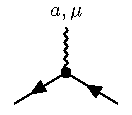
\includegraphics{fig/feynman_diagram/fermion-boson.pdf}
    }
  }
  &=
  ig\gamma^{\mu}t^{a}
  ,
  \\
  \vcenter{
    \hbox{
      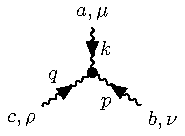
\includegraphics{fig/feynman_diagram/three-boson.pdf}
    }
  }
  &=
  gf^{abc}[g^{\mu\nu}(k-p)^{\rho}+g^{\nu\rho}(p-q)^{\mu}+g^{\rho\mu}(q-k)^{\nu}]
  ,
  \\
  \vcenter{
    \hbox{
      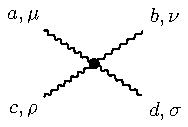
\includegraphics{fig/feynman_diagram/four-boson.pdf}
    }
  }  
  &=
  (\text{very messy }\cdots )
  .
\end{align}

To get these vertex rules, we see the Lagrangian. Consider that the second non-linear interaction term contracts with the state $\ket{k,p,q}$, especially $\partial_{\kappa}A_{\lambda}^{a}$ contracts with $k$, $A^{\kappa b}$ with $p$ and $A^{\lambda c}$ with $q$. We expand the field\footnote{
  Actually, since we did not discuss the canonical quantization of the gauge fields, the discussion below is very naive and sloppy.
} as 
\begin{equation}
  A_{\mu}^{a}(x)
  =
  \int\frac{\dd^3 k'}{(2\pi)^3}
  \left(  
    a_{p,\mu}^{a}e^{-ip\cdot x}
    +
    a_{p,\mu}^{a\dagger}e^{ip\cdot x}    
  \right).
\end{equation}
Therefore, we will get the contribution from that term as
\begin{equation}
  -igf^{abc}(-ik^{\nu})g^{\mu\rho}
  .
\end{equation}

\subsubsection*{Equality of Coupling Constants $g$}

We expect the Feynman amplitude in non-Abelian gauge theories to satisfy the Ward identities, due to the global gauge invariance. Let us check the Ward identities in the simplest case\footnote{
  The Ward identities imply that unphysical polarization states are not produced in scattering processes.
}. In order $g^2$, there are three diagrams. The contribution of the first two diagrams is 
\begin{align}
  i\mathcal{M}_{1,2}^{\mu\nu}\varepsilon_{\mu}^{\ast}(k_{1})\varepsilon_{\nu}^{\ast}(k_{2})
  &=
  (i g)^2 \bar{v}(p_{+})
  \left\{
    \gamma^{\mu}t^{a}\frac{i}{\slashed{p}-\slashed{k}_{2}-m}\gamma^{\nu}t^{b} 
  \right.
  \nonumber
  \\
  &\hspace*{4cm}
  \left.
    +
    \gamma^{\nu}t^{b}
    \frac{i}{\slashed{k}_{2}-\slashed{p}_{+}-m}
    \gamma^{\mu}t^{a}
  \right\}
  u(p)\varepsilon_{\mu}^{\ast}(k_{1})\varepsilon_{\nu}^{\ast}(k_2)
  .
\end{align}
We assume the following conditions:
\begin{itemize}
  \item 
  The polarization of gauge bosons is physical. It implies that the polarization vector should satisfy $k_{i}^{\mu}\varepsilon_{\mu}(k_{i})=0$.
  \item 
  Thus the relations $(\slashed{p}-m)u(p)=0$ and $\bar{v}(p_{+})(-\slashed{p}_{+}-m)=0$ hold.
\end{itemize}
Then we find the non-zero amplitude
\begin{equation}
  i\mathcal{M}_{1,2}^{\mu\nu}\varepsilon_{\mu}^{\ast}(k_{1})k_{2\nu}
  =
  -g^2\bar{v}(p_{+})\gamma^{\mu}u(p)\varepsilon_{1\mu}^{\ast}
  \cdot
  f^{abc}t^{c}
  .
\end{equation}
We have replaced $\varepsilon_{\nu}^{\ast}\rightarrow k_{2\nu}$. This amplitude has the group index structure of a fermion-gauge boson vertex $g\gamma^{\mu}t^{c}$ multiplied by a three gauge boson vertex $gf^{abc}$. 

In the Abelian cases, such a diagram is not permitted because only the fermions-boson vertex exists. Thus the Ward identity holds only the two diagrams in the lowest.

Anyway, in fact, the contribution from a three-gauge boson vertex cancels the amplitude above. Notice that this cancellation takes place only if the value of the coupling constant in the three-boson vertex is identical to that of the fermion-boson vertex. Thus, the coupling constant of all three nonlinear terms in the Yang-Mills Lagrangian must be equal to preserve the Ward identity and avoid the production of bosons with unphysical polarization states.

\subsubsection*{A Flaw in the Argument}

We needed to assume that the second gauge boson was transverse but one might have expected that this information would come out of the argument rather than having to put it in.

Let polarization vector, in general
\begin{equation}
  \varepsilon_{\mu}^{+}(k)
  =
  \left(  
    \frac{k^{0}}{\sqrt{2}|\bm{k|}}
    ,
    \frac{\bm{k}}{\sqrt{2}|\bm{k|}}
  \right)
  ,\ 
  \varepsilon_{\mu}^{-}(k)
  =
  \left(  
    \frac{k^{0}}{\sqrt{2}|\bm{k|}}
    ,
    -
    \frac{\bm{k}}{\sqrt{2}|\bm{k|}}
  \right)
  ,
\end{equation}
where they are parallel to the vector $k=(k^{0},\bm{k})$ and $\tilde{k}=(k^{0},-\bm{k})$. Using this notation, we can obtain no vanishing amplitudes. This leads to another paradox, the optical theorem. 

Clearly, we are missing some crucial elements of the quantum mechanical structure of non-Abelian gauge theories.


\subsection{The Faddeev-Popov Lagrangian}

First consider the quantization of the pure gauge theory, without fermions. Let us constrain the gauge directions by applying a gauge-fixing condition $G(A)=0$ at each space-time point $x$.

We will insert the identity
\begin{equation}
  1
  =
  \int\mathcal{D}\alpha(x)\ 
  \delta(G(A^{\alpha}))
  \det\left( \frac{\delta G(A^{\alpha})}{\delta\alpha} \right)
\end{equation}
to converge the path integral. It was introduced by Faddeev and Popov. Here $A^{\alpha}$ is the transformed gauge field
\begin{equation}
  (A^{\alpha})^{a}_{\mu}
  =
  A_{\mu}^{a}+\frac{1}{g}D_{\mu}\alpha^{a}
  ,
\end{equation}
where $D_{\mu}$ is the covariant derivative acting on a field in the adjoint representation. This shift does not change the measure 
\begin{equation}
  \mathcal{D}A
  =
  \prod_{x}\prod_{a,\mu}\dd A^{a}_{\mu}
  ,
\end{equation}
so we obtain the relation
\begin{equation}
  \int\mathcal{D}A\ e^{iS[A]}
  =
  \left(  
    \int\mathcal{D}\alpha
  \right)
  \int\mathcal{D}A\ 
  e^{iS[A]}\delta(G(A))
  \det\left( \frac{\delta G(A^{\alpha})}{\delta\alpha} \right)
  ,
\end{equation}
where the integration of the field $\alpha$ is factored out since the integrand has no dependence on $\alpha$. From this point, the manipulations of the Abelian cases lead to the gauge field propagator
\begin{equation}
  \ev*{
    A_{\mu}^{a}(x)A_{\nu}^{b}(y)
  }
  =
  \int\frac{\dd^4 k}{(2\pi)^4}
  \frac{-i}{k^2+i\varepsilon}
  \left(  
    g_{\mu\nu}
    -
    (1-\xi)
    \frac{k_{\mu}k_{\nu}}{k^2}
  \right)
  \delta^{ab}e^{-ik\cdot(x-y)}
  ,
\end{equation}
with a freely adjustable gauge parameter $\xi$.

Here there is one more nontrivial ingredient unlike in the case of QED. That is the functional determinant of
\begin{equation}
  \frac{\delta G(A^{\alpha})}{\delta\alpha}
  =
  \frac{1}{g}\partial^{\mu}D_{\mu}
  ,
\end{equation}
where it has an explicit dependence on $A$. Faddeev and Popov represent this determinant by introducing the new fermionic field $c$ as
\begin{equation}
  \det\left( \frac{1}{g}\partial^{\mu}D_{\mu} \right)
  =
  \int\mathcal{D}c\mathcal{D}\bar{c}\ 
  \exp\left[ i\int\dd^4 x\ \bar{c}(-\partial^{\mu}D_{\mu})c \right]
  .
\end{equation}
$c$ and $\bar{c}$ are anticommuting fields but they are transformed as scalars under the Lorentz transformation. These new fields are called \textit{Faddeev-Popov ghosts}.

We write the ghost Lagrangian
\begin{equation}
  \mathcal{L}
  =
  \bar{c}^{a}
  \left(  
    -
    \partial^2 \delta^{ac}
    -
    g\partial^{\mu}f^{abc}A_{\mu}^{b}
  \right)
  c^{c}
\end{equation}
and it gives the Feynman rules
\begin{align}
  \text{propagator\ (updating)}\ 
  &=
  \frac{i\delta^{ab}}{p^2}
  ,
  \\
  \text{vertex\ (updating)}\ 
  &=
  -gf^{abc}p^{\mu}
  .
\end{align}
Thus the final Lagrangian is 
\begin{equation}
  \mathcal{L}
  =
  -
  \frac{1}{4}
  (F_{\mu\nu}^{a})^2
  -
  \frac{1}{2\xi}(\partial^{\mu}A_{\mu}^{a})^2
  +
  \bar{\psi}(i\slashed{D}-m)\psi
  +
  \bar{c}^{a}
  \left(  
    -
    \partial^2 \delta^{ac}
    -
    g\partial^{\mu}f^{abc}A_{\mu}^{b}
  \right)
  c^{c}
  .  
\end{equation}

\begin{itemize}
  \item 
  We can derive the Feynman diagram expansion of any correlation function in a non-Abelian gauge theory.
  \item 
  $S$-matrix elements are gauge invariant.
\end{itemize}


\subsection{Ghosts and Unitarity}

The diagrams which violate the optical theorem are
\begin{equation}
  \vcenter{
    \hbox{
      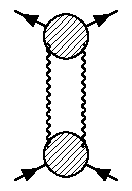
\includegraphics{fig/feynman_diagram/opt_thm.pdf}
    }
  }  
  .
\end{equation}
We can prove the ghost diagram cancels such a contribution\footnote{
  Note! I have to prepare a better one.
}:
\begin{equation}
  \vcenter{
    \hbox{
      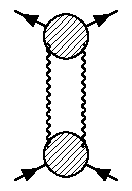
\includegraphics{fig/feynman_diagram/opt_thm.pdf}
    }
  }  
  +  
  \vcenter{
    \hbox{
      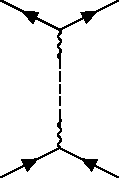
\includegraphics{fig/feynman_diagram/opt_thm_ghost.pdf}
    }
  }  
  .
\end{equation}
This example illustrates a general physical interpretation of FP ghost. These "particles" serve as negative degrees of freedom to cancel the effect of the unphysical timelike and longitudinal state of the gauge bosons. 


\subsection{BRST symmetry}

We rewrite the Faddeev-Popov Lagrangian with new commuting scalar fields $B^{a}$:
\begin{equation}
  \mathcal{L}
  =
  -\frac{1}{4}
  (F_{\mu\nu}^{a})^2
  +
  \bar{\psi}(i\slashed{D}-m)\psi
  +
  \frac{\xi}{2}(B^{a})^2
  +
  B^{a}\partial^{\mu}A_{\mu}^{a}
  +
  \bar{c}^{a}(-\partial^{\mu}D_{\mu}^{ac})c^{c}
  .
  \label{eqn:brst_lagrangian}
\end{equation}
The new field $B^{a}$ has a quadratic term without derivatives, so it is not a normal propagating field, called an \textit{auxiliary field}. 

Consider the following infinitesimal transformation:
\begin{align}
  \delta A_{\psi}^{a}
  &=
  \varepsilon D_{\mu}^{ac}c^{c}
  ,
  \\
  \delta\psi
  &=
  ig\varepsilon c^{a}t^{a}\psi
  ,
  \\
  \delta c^{a}
  &=
  -
  \frac{1}{2}g\varepsilon f^{abc}c^{b}c^{c}
  ,
  \\
  \delta \bar{c}^{a}
  &=
  \varepsilon B^{a}
  ,
  \\
  \delta B^{a}
  &=
  0
  ,
\end{align}
where $\varepsilon$ is a parameter. We can prove that the gauge-fixing Lagrangian \eqref{eqn:brst_lagrangian} is invariant under the above transformations. The first two terms are invariant since the transformation law of $A_{\mu}^{a}$ and $\psi$ is the local gauge symmetry. The third term is also invariant apparently. The deformation of the last term will vanish by the Jacobi identity.









\subsection{Quantum Chromodynamics}








\clearpage
\appendix
\section{Some notes}

\subsection{Normalization of Maxwell Lagrangian}

The Maxwell lagrangian is the form
\begin{equation}
  \mathcal{L}
  =
  NF^{\mu\nu}F_{\mu\nu}
\end{equation}
where $F^{\mu\nu}=\partial^{\mu}A^{\nu}-\partial^{\nu}A^{\mu}$ is a field strength. We will determine the constant $N$ to lagrangian contains the term 
\begin{equation}
  \mathcal{L}
  =
  \frac{1}{2}\dot{A}_{1}^2
  +
  \frac{1}{2}\dot{A}_{2}^2
  +
  \frac{1}{2}\dot{A}_{3}^2
  +
  \cdots
  \ .
\end{equation}
Now expanding the term $F^{\mu\nu}F_{\mu\nu}$ carefully, we obtain
\begin{align}
  F^{\mu\nu}F_{\mu\nu}
  &=
  (\partial^{\mu}A^{\nu}-\partial^{\nu}A^{\mu})
  (\partial_{\mu}A_{\nu}-\partial_{\nu}A_{\mu})
  \nonumber
  \\
  &=
  2((\partial^{\mu}A^{\nu})(\partial_{\mu}A_{\nu})-(\partial_{\mu}A^{\nu})(\partial_{\nu}A_{\mu}))
  \nonumber
  \\
  &=
  -2(\dot{A}_{1}^2+\dot{A}_{2}^2+\dot{A}_{3}^2)+\cdots
\end{align}
and thus, the constant $N$ satisfies the condition $-2N=1/2$ and $N=-1/4$. That's why we get Maxwell Lagrangian as
\begin{equation}
  \mathcal{L}
  =
  -\frac{1}{4}F^{\mu\nu}F_{\mu\nu}
  \ .
\end{equation}



\clearpage
\bibliography{hoge}
\bibliographystyle{ytphys}

\nocite{Peskin_IntroductionQuantum_1995}
\nocite{Wess_SupersymmetrySupergravity_1992}


\end{document}
